\documentclass[border=2pt]{standalone}
\usepackage{amsmath}
\usepackage{tikz}
\usetikzlibrary{intersections}
\usetikzlibrary{arrows}
\usetikzlibrary{quotes,angles}
\usepackage{amsmath}
\usepackage{xcolor}

\begin{document}

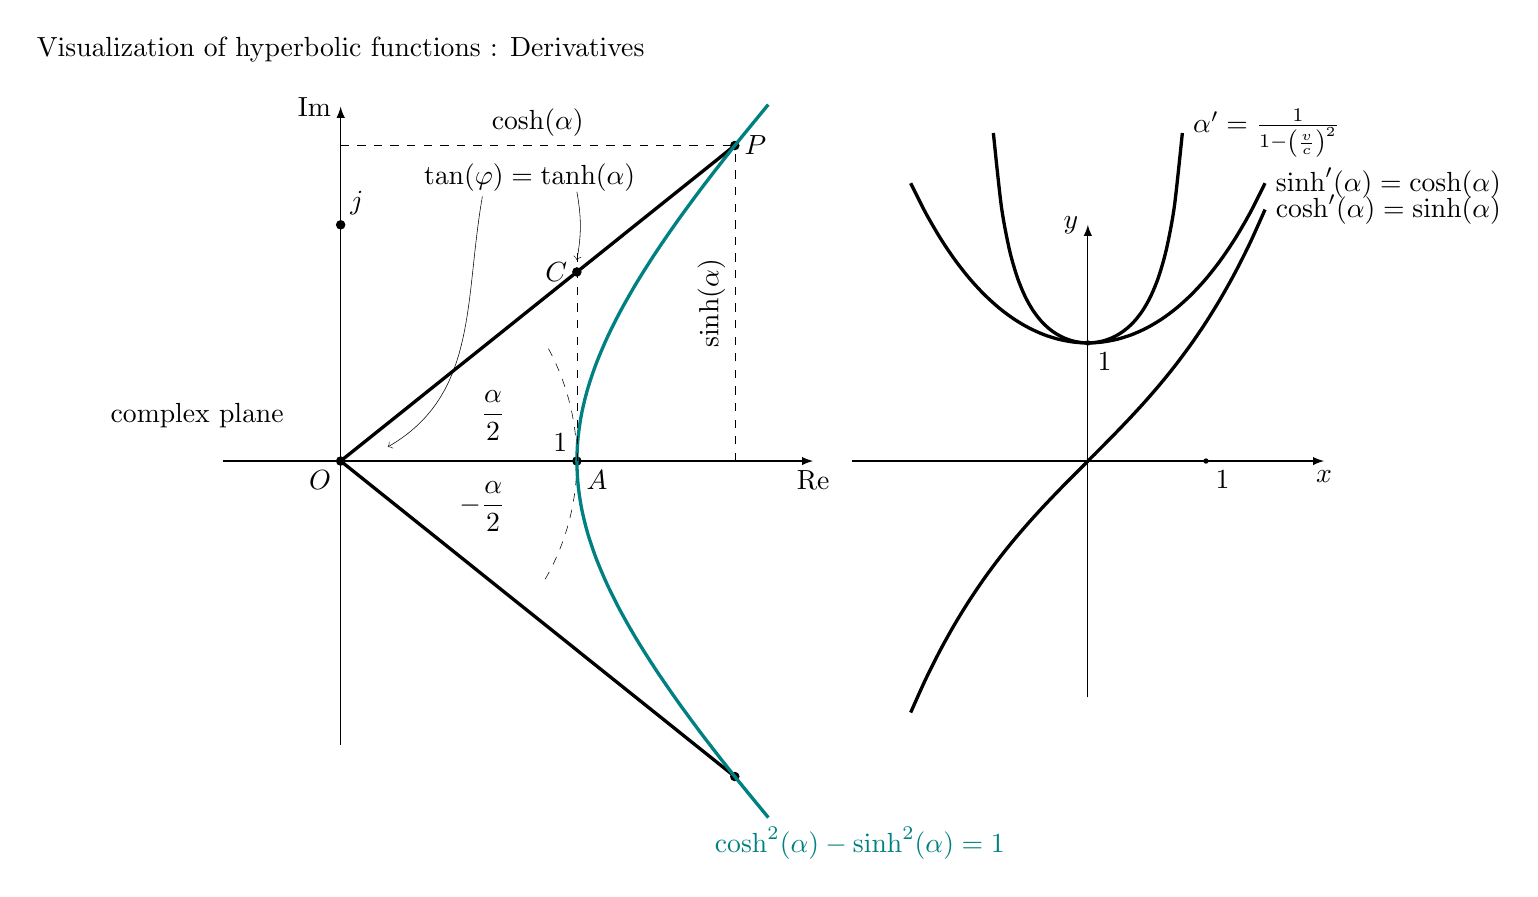
\begin{tikzpicture}[scale=3.0]

% Draw x and y axis lines
\draw [->,>=latex] (-0.5,0) -- (2.00,0) node [below] {$\mathrm{Re}$};
\draw [->,>=latex] (0,-1.2) -- (0,1.50) node [left ] {$\mathrm{Im}$};
\node[above left] at (-0.2, 0.1) {complex plane};
\filldraw[black] (1,0) circle (0.5pt) node[above left ] {$1$} node[below right] {$A$} ;
\filldraw[black] (0,1) circle (0.5pt) node[above right] {$j$} ;
\filldraw[black] (0,0) circle (0.5pt) node[below left ] {$O$} ;
\node[above] at (0.0,1.65) {Visualization of hyperbolic functions : Derivatives};

% Draw a circle at the origin of radius 1
%\draw (0,0) circle (1);
\draw [very thin, dashed] ({cos(-30)},{sin(-30)}) arc (-30:30:1) ;

%\draw [very thin, dashed] (-1.5,-1.5) -- ( 1.5, 1.5) node[above] {$y=x$} ;
%\draw [very thin, dashed] (-1.5, 1.5) -- ( 1.5,-1.5) ;

\pgfmathsetmacro{\angle}{1.1}
\pgfmathsetmacro{\length}{\angle}
\pgfmathsetmacro{\anglevarphi}{atan(tanh(\angle))}

\filldraw[black] ({ cosh(\angle)}, { sinh(\angle)}) circle (0.5pt) node[right] {$P$} ;
\filldraw[black] ({ cosh(\angle)}, {-sinh(\angle)}) circle (0.5pt) ;

\draw [very thin, dashed] ( 0.0, { sinh(\angle)}) -- node[above] {$\cosh(\alpha)$}  ({ cosh(\angle)}, { sinh(\angle)}) ;
\draw [very thin, dashed] ( { cosh(\angle)}, 0.0) -- node[above, rotate=90] {$\sinh(\alpha)$}  ( { cosh(\angle)}, { sinh(\angle)}) ;

\draw[very thick] (0,0) -- ({ cosh(\angle)}, { sinh(\angle)}) ;
\draw[very thick] (0,0) -- ({ cosh(\angle)}, {-sinh(\angle)}) ;


% 画双曲线
\draw[very thick,smooth,variable=\x, teal] plot[domain=-\angle-0.1:\angle+0.1] ({ cosh(\x)}, {sinh(\x)}) ;
\node[below right, teal] at ({ cosh(\angle-0.1)}, {-sinh(\angle+0.1)}) {$\cosh^2(\alpha) - \sinh^2(\alpha) = 1$} ;
%\draw[very thick,smooth,variable=\x, teal] plot[domain=-1.2:1.2] ({-cosh(\x)}, {sinh(\x)}) ;



\node[above=4pt ] at (0.6, 0) {$\;\;\:\dfrac{\alpha}{2}$} ;
\node[below=4pt ] at (0.6, 0) {$ -\dfrac{\alpha}{2}$} ;


\draw [very thin, dashed] (1, 0)  -- (1, { tanh(\angle)+0.1}) ;
\filldraw[black] ( 1, { tanh(\angle)}) circle (0.5pt) node[left ] {$C$} ;
\draw [very thin, ->] (0.8, 1.1) node[above ] {$\tan(\varphi) = \tanh(\alpha)$} (1.0, 1.14) to [out=280,in=80] ( 1, { tanh(\angle) + 0.05}) ;
\draw [very thin, ->] (0.60, 1.12) to [out=260,in=30] (0.20, 0.06) ;

\begin{scope}[xshift=90, scale=0.5]

\draw [->,>=latex] (-2.0,0) -- (2.00,0) node [below] {$x$};
\draw [->,>=latex] (0,-2.0) -- (0,2.00) node [left ] {$y$};
\filldraw[black] (1,0) circle (0.5pt) node[below right] {$1$} ;
\filldraw[black] (0,1) circle (0.5pt) node[below right] {$1$} ;

\draw[very thick,smooth,variable=\x] plot[domain=-0.8:0.8] ({ \x}, {1/(1- \x * \x)}) node[right] {$\alpha '=\frac{1}{1-\left(\frac{v}{c}\right)^2}$} ;
\draw[very thick,smooth,variable=\x] plot[domain=-1.5:1.5] ({ \x}, { cosh(\x)}) node[right] {$\sinh'(\alpha)=\cosh(\alpha)$} ;
\draw[very thick,smooth,variable=\x] plot[domain=-1.5:1.5] ({ \x}, { sinh(\x)}) node[right] {$\cosh'(\alpha)=\sinh(\alpha)$} ;

\end{scope}

\end{tikzpicture}

\end{document}
